%!TEX root = CVPR_2018_Nonlinear_3DMM.tex
\Section{Experimental Results}
\label{sec:exp}

The experiments study three aspects of the proposed nonlinear 3DMM, in terms of its expressiveness, representation power, and applications to facial analysis.
Using facial mesh triangle definition by Basel Face Model~(BFM)~\cite{paysan20093d}, we train our 3DMM using 300W-LP dataset~\cite{zhu2016face}. 
The model is optimized using Adam optimizer with an initial learning rate of $0.001$ when minimizing $L_0$, and $0.0002$ when minimizing $L$.
We set the following parameters: $Q=53,215$, $U=V=128$, $l_S=l_T=160$. $\lambda$~values are set to make losses to have similar magnitudes.


\SubSection{Expressiveness}
\Paragraph{Exploring feature space}
We use the entire CelebA dataset~\cite{liu2015faceattributes} with ${\sim}200$k images to feed to our network to obtain the empirical distribution of our shape and texture parameters. 
By varying the mean parameter along each dimension proportional to their standard deviations, we can get a sense how each element contributes to the final shape and texture.
We sort elements in the shape parameter $\mathbf{f}_S$ based on their differences to the mean 3D shape. 
Fig.~\ref{fig:varying_shape} shows four examples of shape changes, whose differences rank No.$1$, $40$, $80$, and $120$ among $160$ elements.
%
Most of top changes are expression related.
Similarly, in Fig.~\ref{fig:varying_tex}, we visualize different texture changes by adjusting only one element of $\mathbf{f}_T$ off the mean parameter $\bar{\mathbf{f}}_T$.
The elements with the same $4$ ranks as the shape counterpart are selected.


\begin{figure}[t!]

\begin{center}
\small
\setlength{\tabcolsep}{3pt}
  \resizebox{0.8\linewidth}{!}{
\begin{tabular}{ @{}c@{}c@{}c@{}c@{}c@{}c@{}c@{}c@{}}
%\toprule
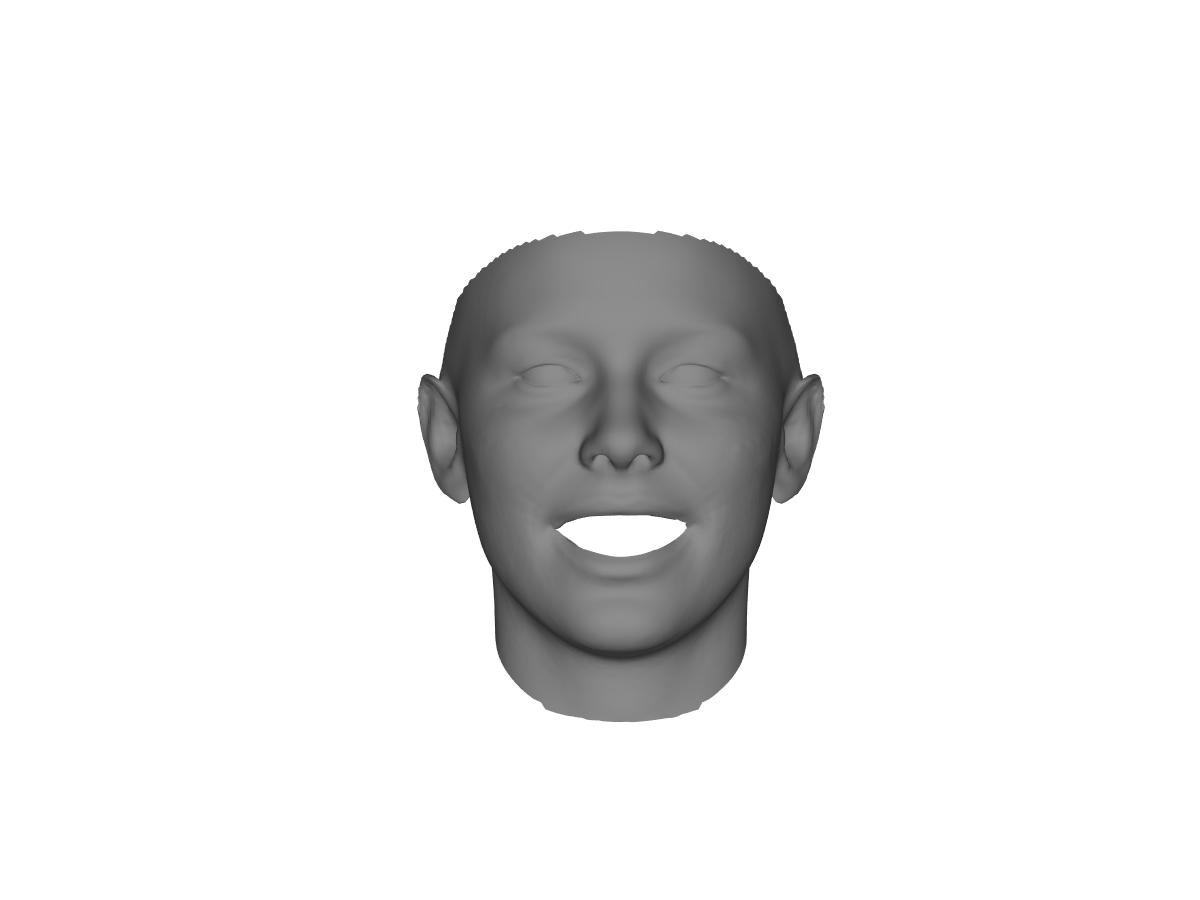
\includegraphics[trim=400 180 370 230,clip,width=\VaryingShapeFigWid]{img/Basis/pred_shape_30_pos.jpg} &
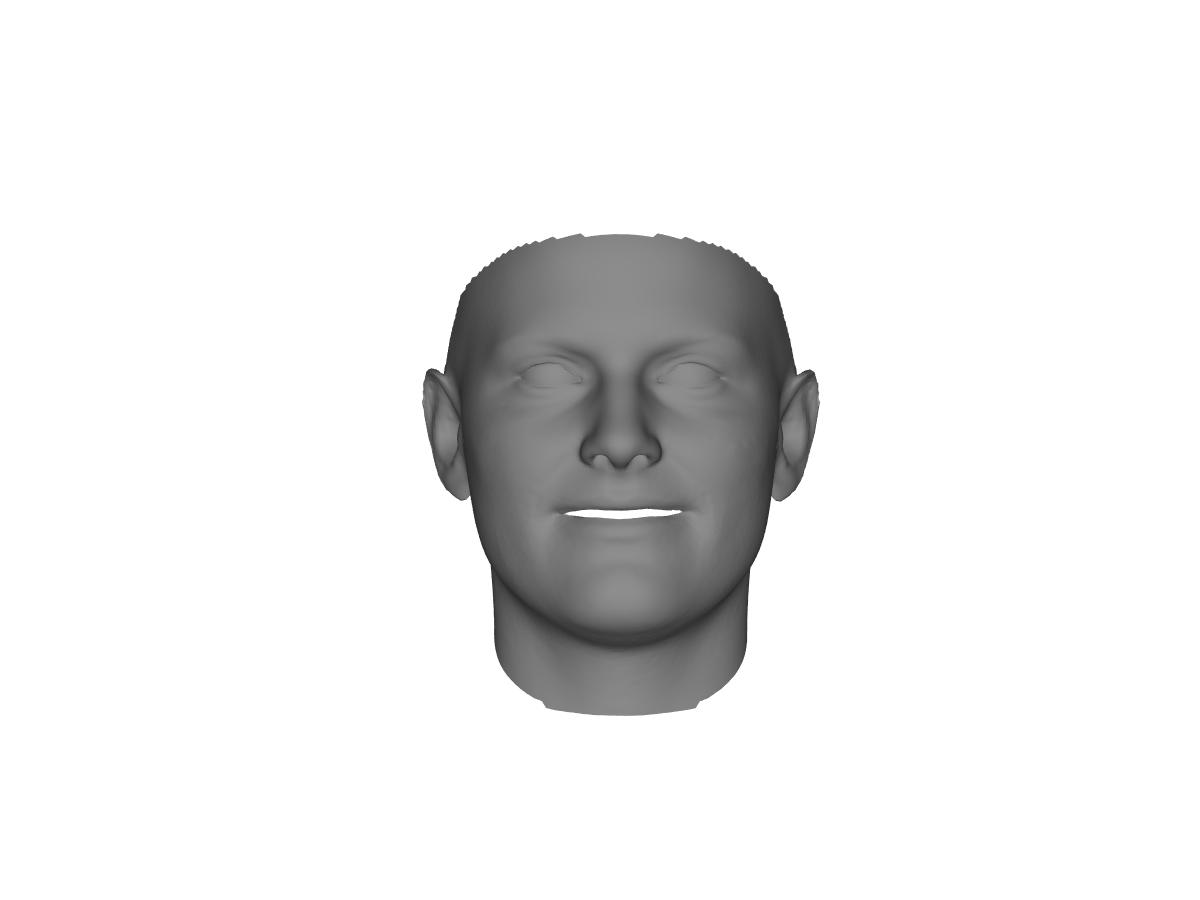
\includegraphics[trim=400 180 370 230,clip,width=\VaryingShapeFigWid]{img/Basis/pred_shape_6_pos.jpg} &
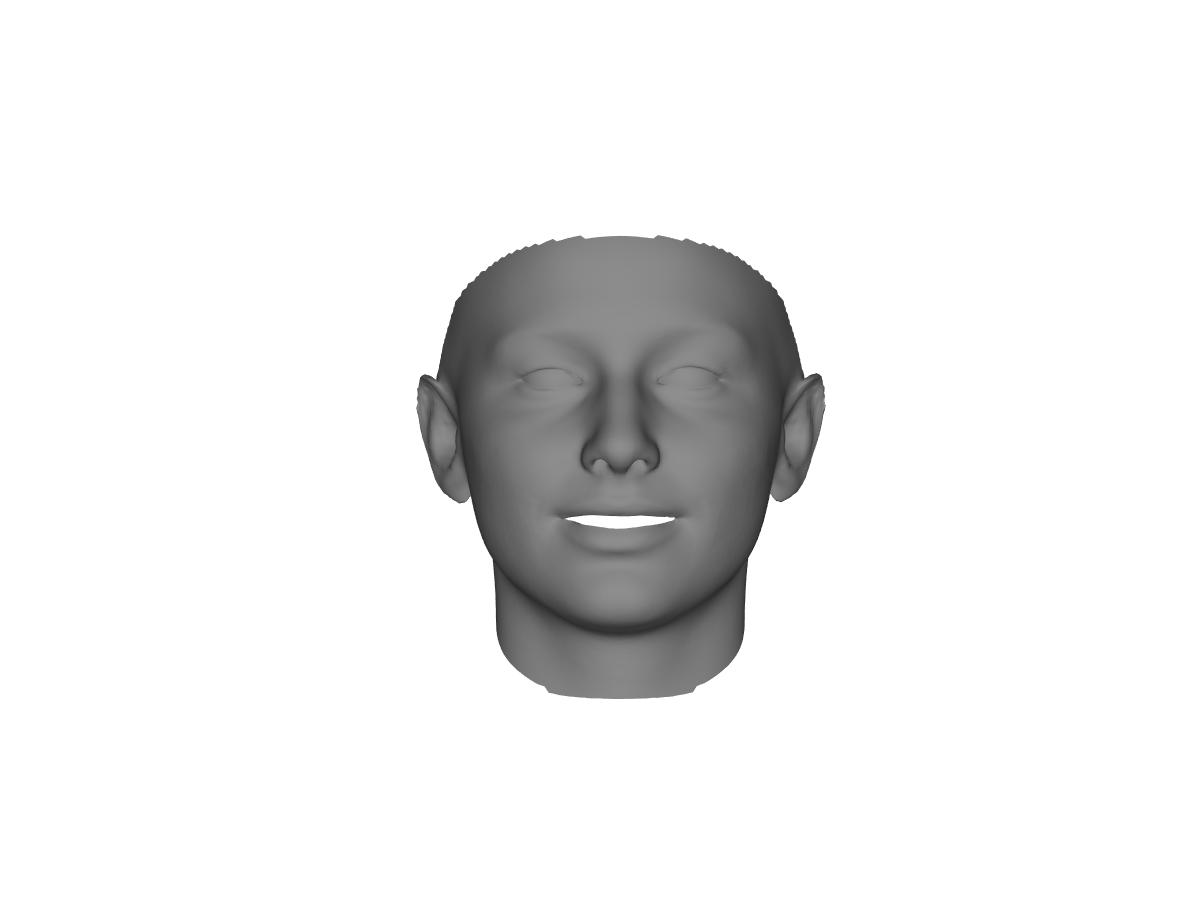
\includegraphics[trim=400 180 370 230,clip,width=\VaryingShapeFigWid]{img/Basis/pred_shape_31_pos.jpg} &
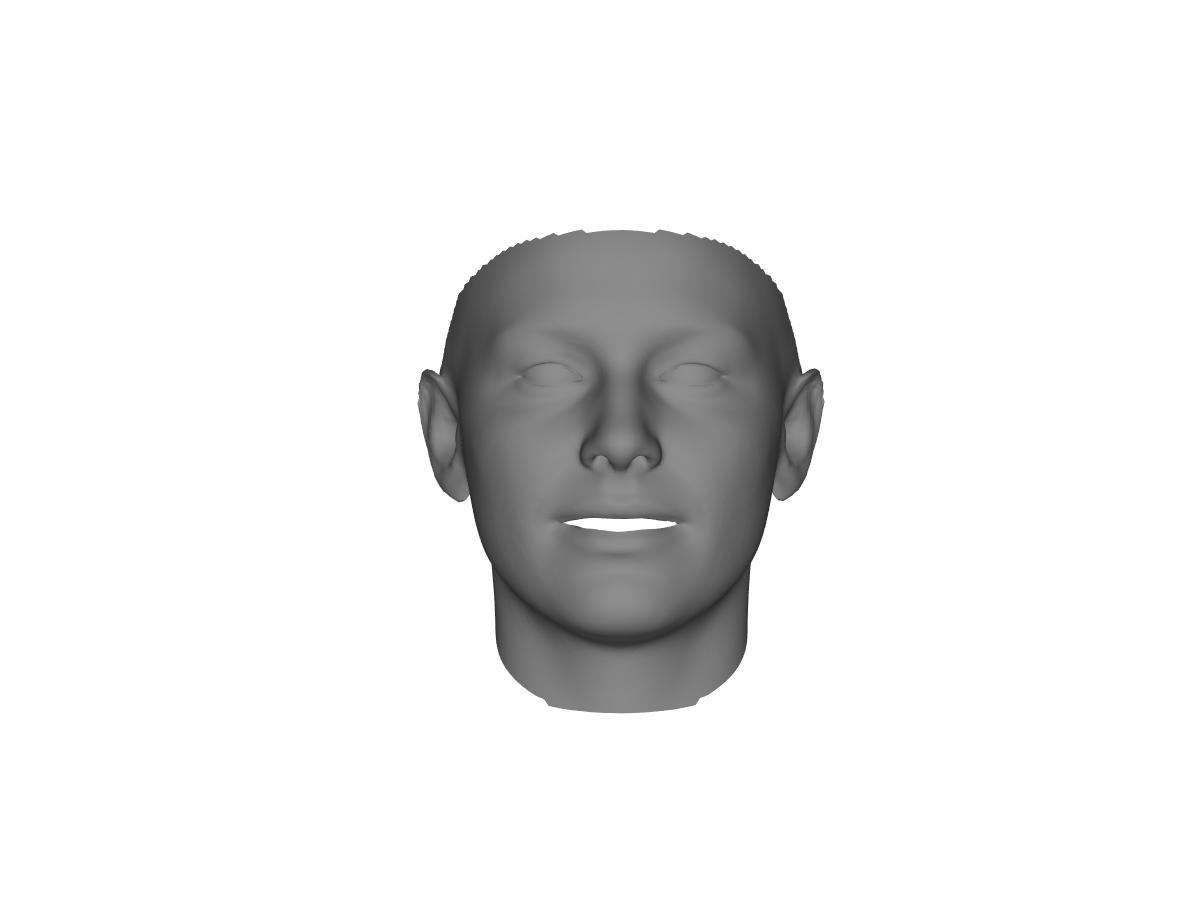
\includegraphics[trim=400 180 370 230,clip,width=\VaryingShapeFigWid]{img/Basis/pred_shape_135_pos.jpg} &
\\
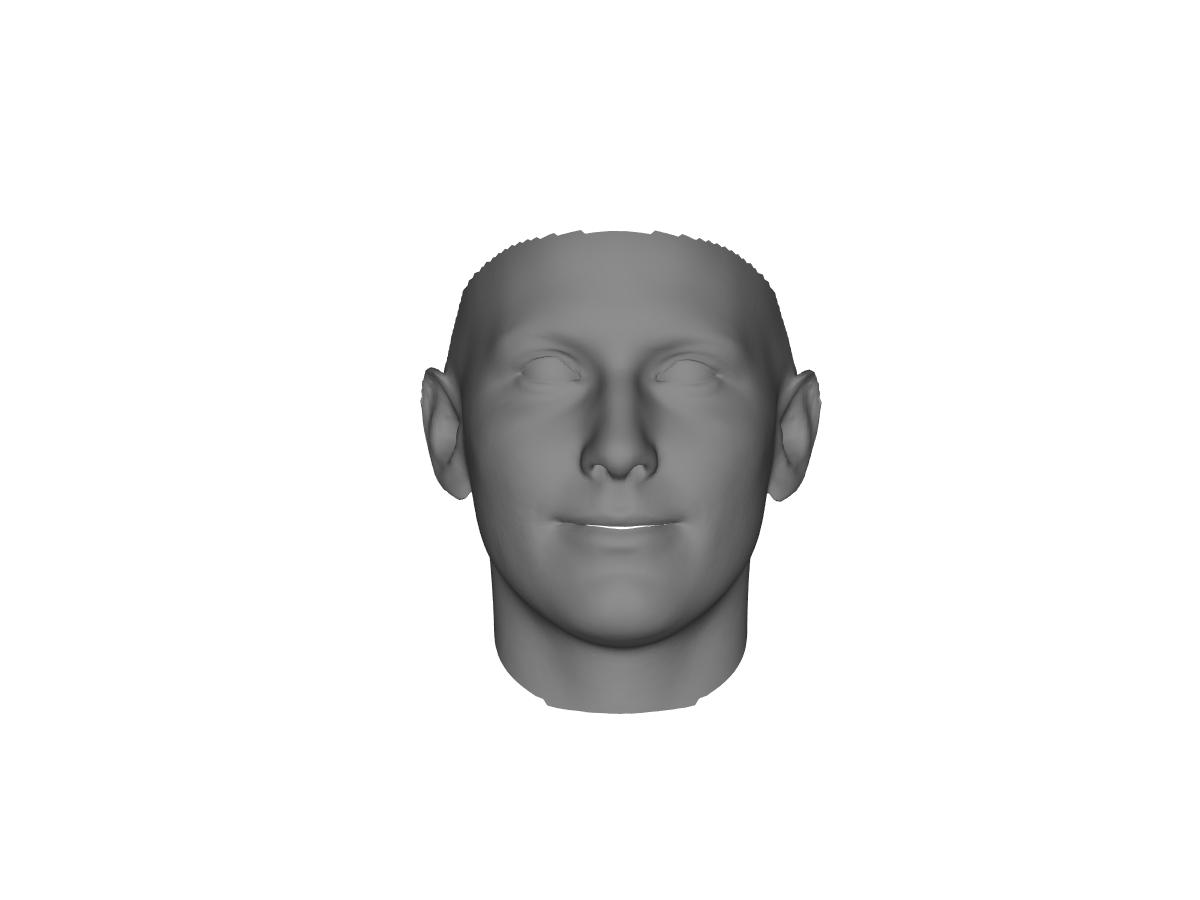
\includegraphics[trim=400 180 370 230,clip,width=\VaryingShapeFigWid]{img/Basis/pred_shape_133_neg.jpg} &
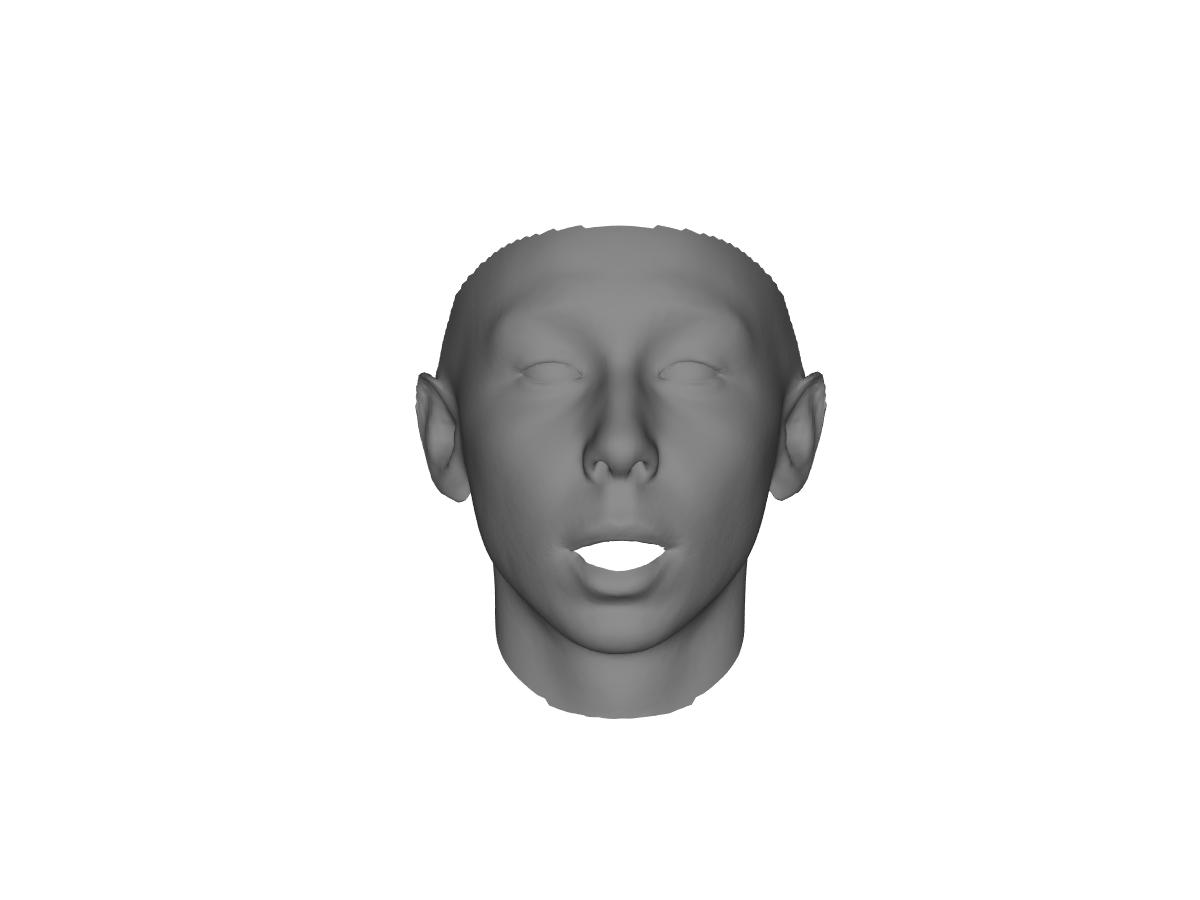
\includegraphics[trim=400 180 370 230,clip,width=\VaryingShapeFigWid]{img/Basis/pred_shape_6_neg.jpg} &
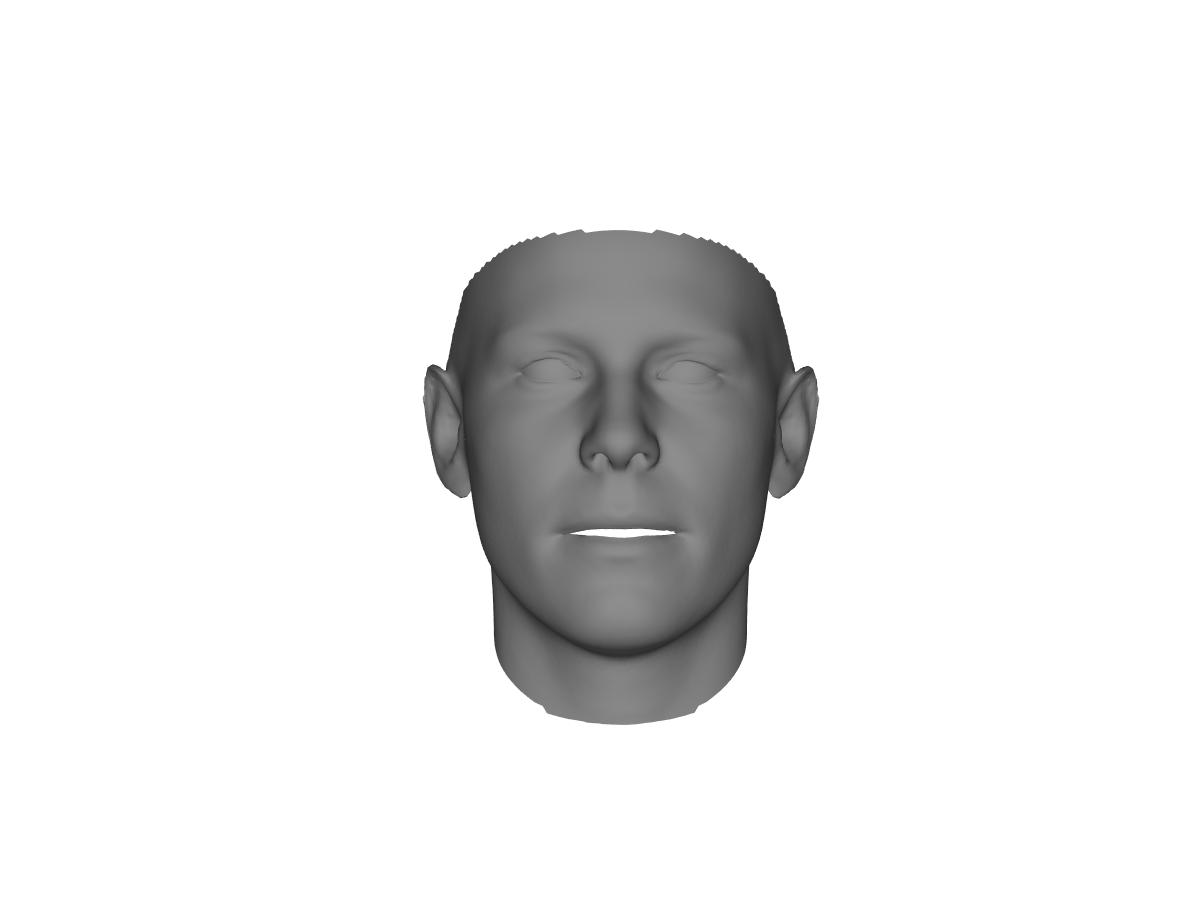
\includegraphics[trim=400 180 370 230,clip,width=\VaryingShapeFigWid]{img/Basis/pred_shape_31_neg.jpg} &
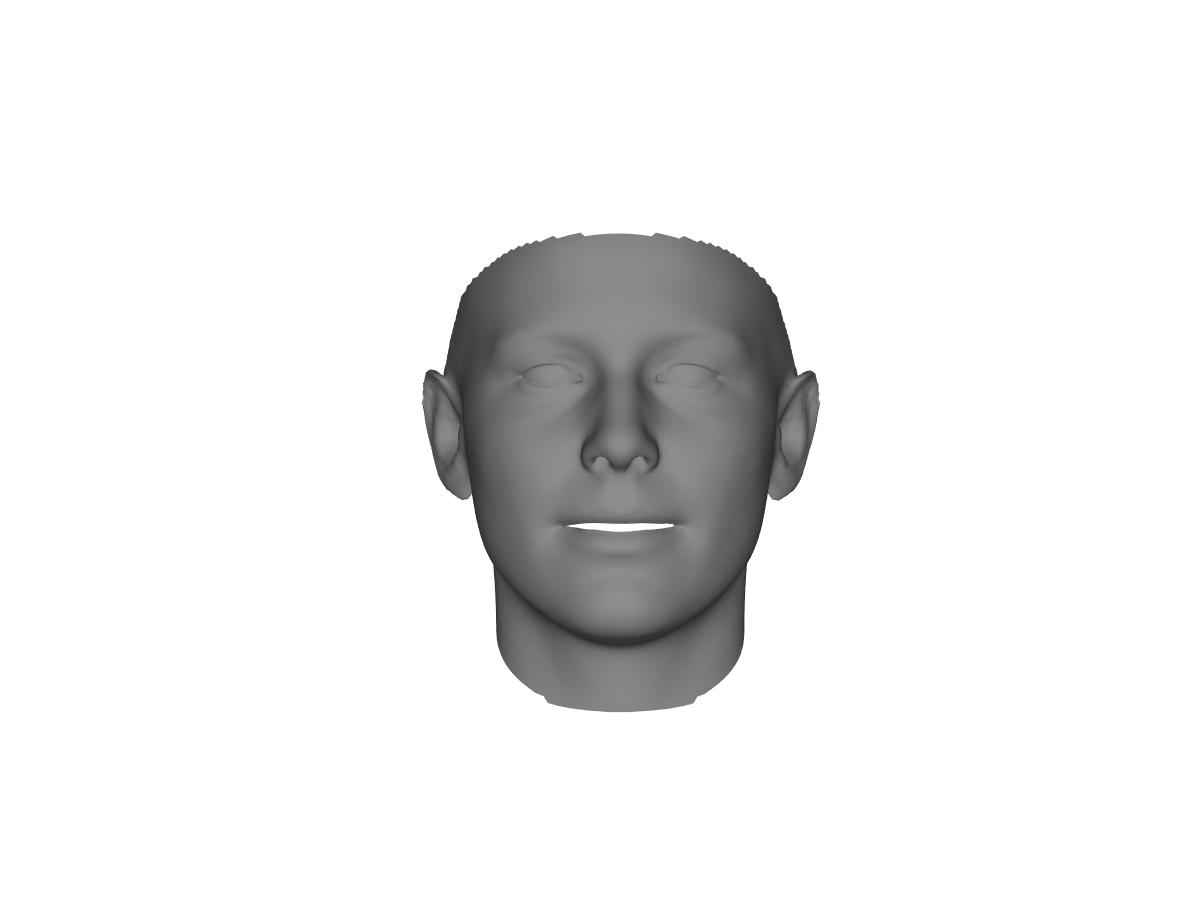
\includegraphics[trim=400 180 370 230,clip,width=\VaryingShapeFigWid]{img/Basis/pred_shape_135_neg.jpg} &
\end{tabular}
}
\vspace{-2mm}
\caption{\small Each column shows shape changes when varying one element of $\mathbf{f}_S$. Ordered by the magnitude of shape changes.}
\label{fig:varying_shape}\figvspace \vspace{-2mm}
\end{center}

\end{figure}


\begin{figure}[t!]
\begin{center}
\small
\setlength{\tabcolsep}{3pt}
  \resizebox{0.8\linewidth}{!}{
\begin{tabular}{ @{}c@{}c@{}c@{}c@{}c@{}c@{}c@{}c@{}}
%\toprule
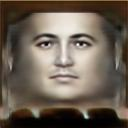
\includegraphics[width=\VaryingShapeFigWid]{img/Basis/pred_tex_105_pos.jpg} &
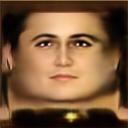
\includegraphics[width=\VaryingShapeFigWid]{img/Basis/pred_tex_66_pos.jpg} &
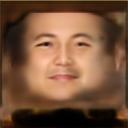
\includegraphics[width=\VaryingShapeFigWid]{img/Basis/pred_tex_34_pos.jpg} &
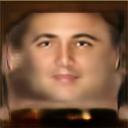
\includegraphics[width=\VaryingShapeFigWid]{img/Basis/pred_tex_134_pos.jpg} &
\\
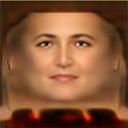
\includegraphics[width=\VaryingShapeFigWid]{img/Basis/pred_tex_105_neg.jpg} &
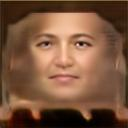
\includegraphics[width=\VaryingShapeFigWid]{img/Basis/pred_tex_66_neg.jpg} &
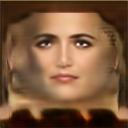
\includegraphics[width=\VaryingShapeFigWid]{img/Basis/pred_tex_34_neg.jpg} &
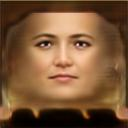
\includegraphics[width=\VaryingShapeFigWid]{img/Basis/pred_tex_134_neg.jpg} &
\end{tabular}
}
\vspace{-2mm}
\caption{\small Each column shows texture changes when varying one element of $\mathbf{f}_T$.}
\label{fig:varying_tex}\figvspace \vspace{-2mm}
\end{center}
\end{figure}



\Paragraph{Attribute Embedding}
To better understand different shape and texture instances embedded in our two decoders, we dig into their attribute meaning.
For a given attribute, e.g., male, we feed images with that attribute $\{\mathbf{I}_i\}_{i=1}^n$ into our encoder to obtain two sets of parameters $\{\mathbf{f}_S^{i}\}_{i=1}^n$ and $\{\mathbf{f}_T^{i}\}_{i=1}^n$. 
These sets represent corresponding empirical distributions of the data in the low dimensional spaces. 
By computing the mean parameters $\mathbf{\bar{f}}_S, \mathbf{\bar{f}}_T$, and feed into their respective decoders, we can reconstruct the mean shape and texture with that attribute. Fig.~\ref{fig:meaningful_basis} visualizes the reconstructed shape and texture related to some attributes. 
Differences among attributes present in both shape and texture.

\begin{figure}[t!]
\begin{center}
\small
\setlength{\tabcolsep}{3pt}
\begin{tabular}{ @{\hskip 1.5mm}c@{}c@{\hskip 1.5mm}c@{}c@{}c@{}c@{}c@{\hskip 1.5mm}c@{}}
%\toprule
\multicolumn{2}{c}{Male} & \multicolumn{2}{c}{Mustache} & \multicolumn{2}{c}{Pale skin} \\
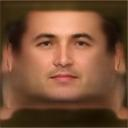
\includegraphics[width=\afifthcolumn]{img/representation/pred_tex_Male.jpg} &
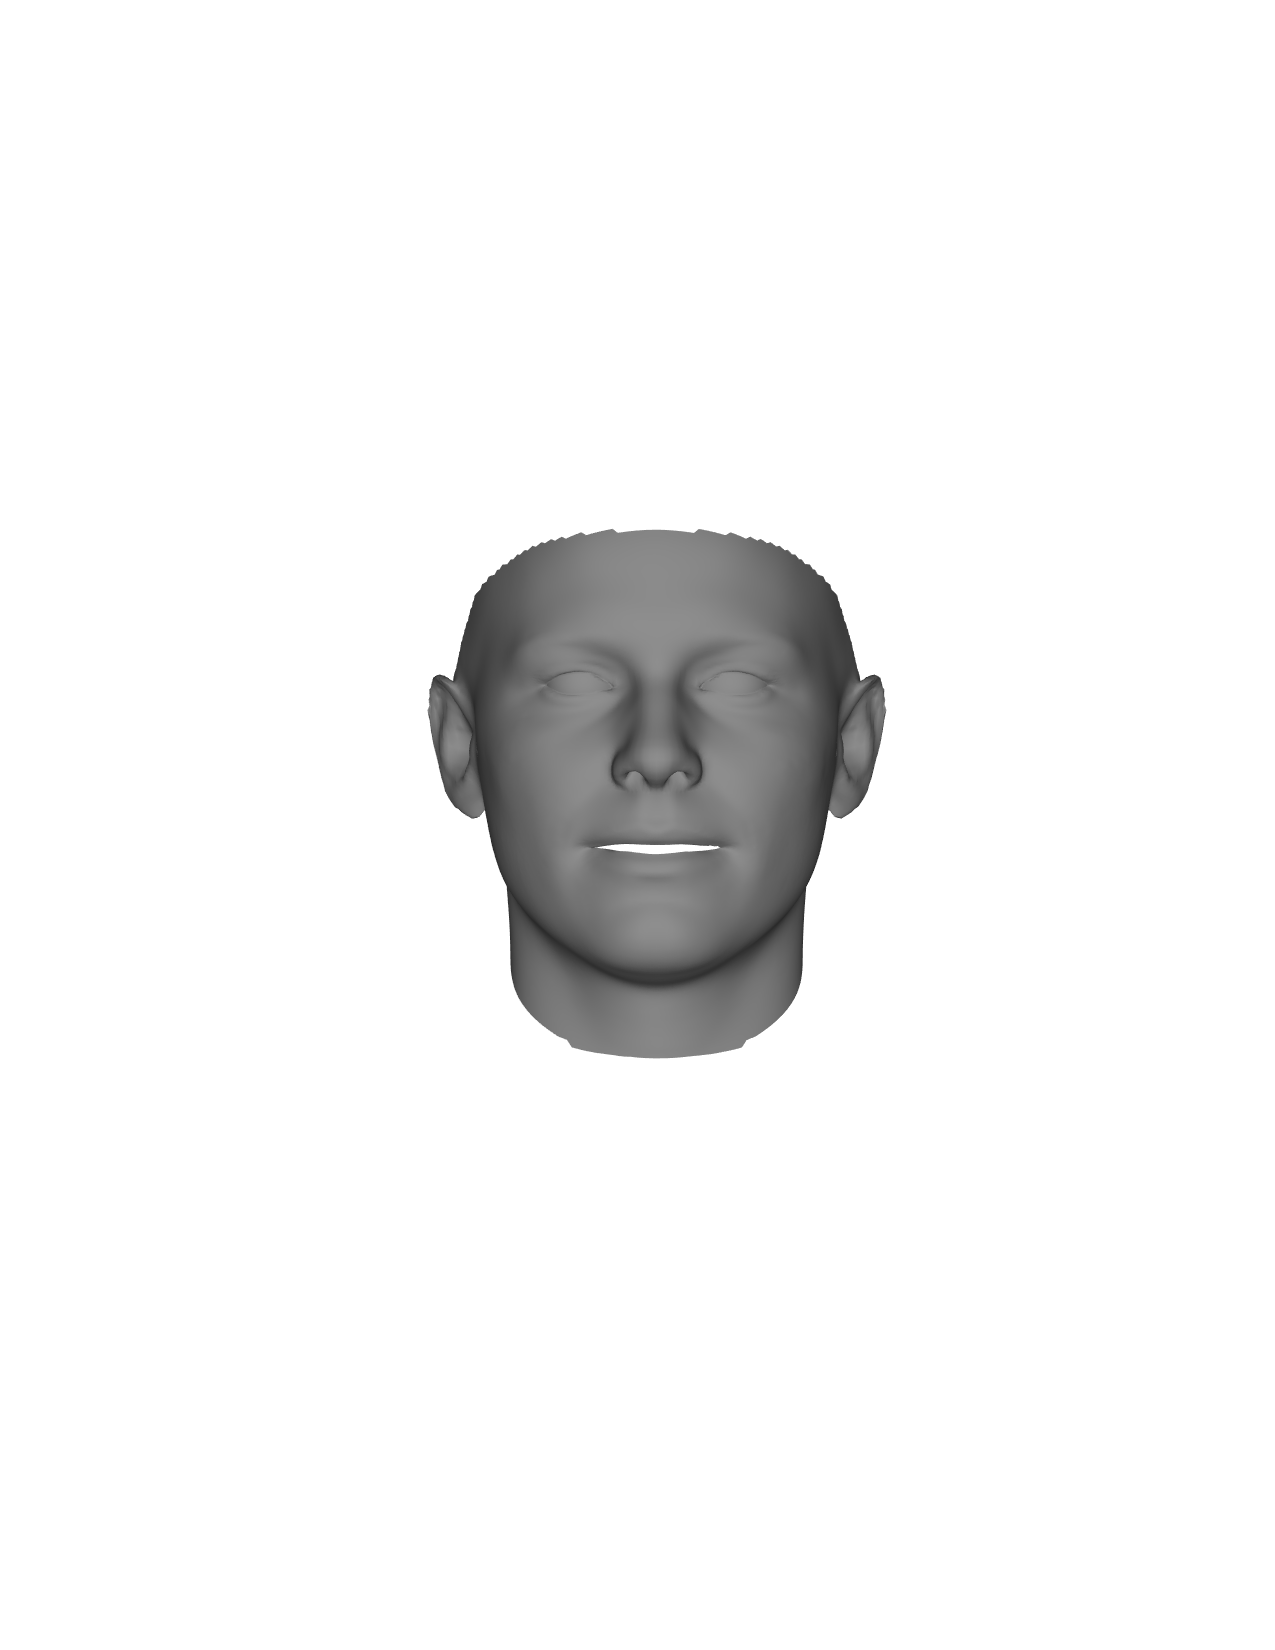
\includegraphics[trim=150 250 150 250,clip, width=\afifthcolumn]{img/representation/pred_shape_Male.pdf} &
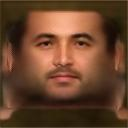
\includegraphics[width=\afifthcolumn]{img/representation/pred_tex_Mustache.jpg} &
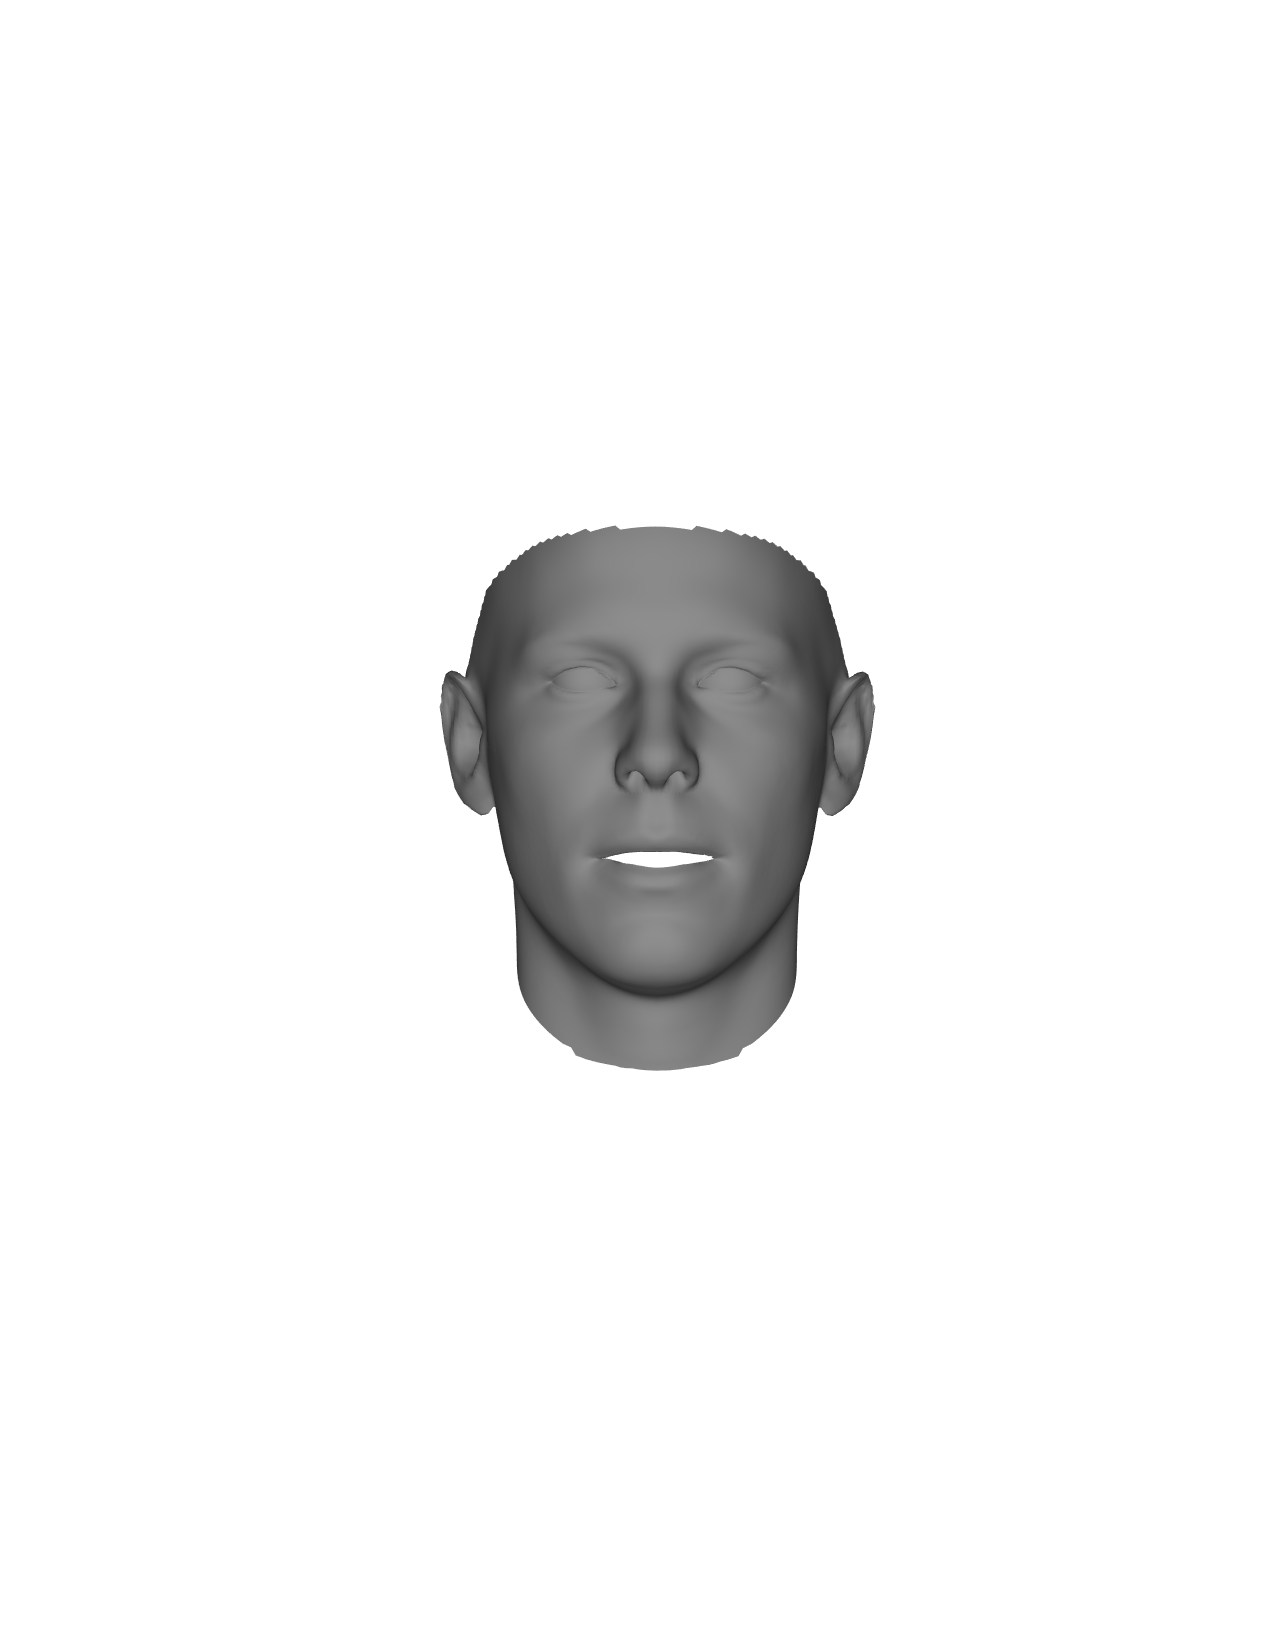
\includegraphics[trim=150 250 150 250,clip, width=\afifthcolumn]{img/representation/pred_shape_Mustache.pdf} &
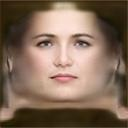
\includegraphics[width=\afifthcolumn]{img/representation/pred_tex_Pale_Skin.jpg} &
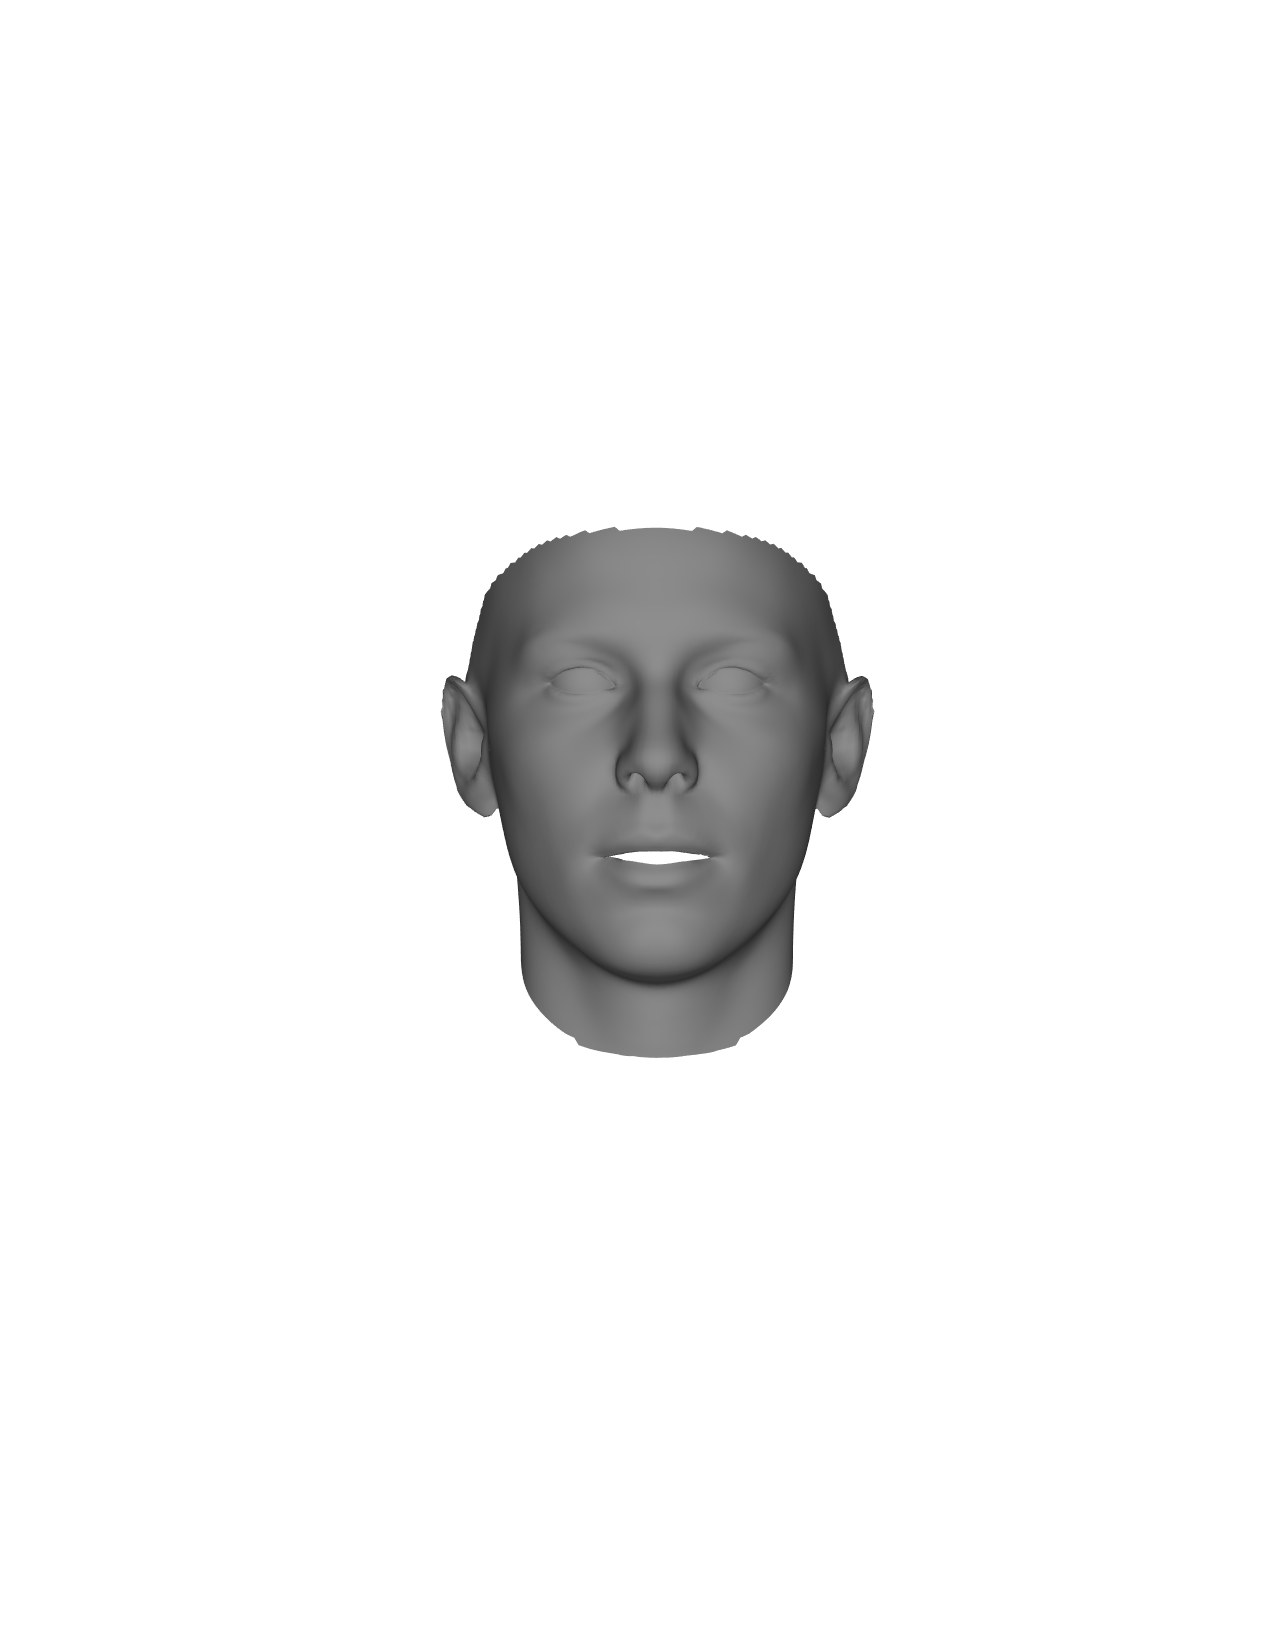
\includegraphics[trim=150 250 175 250,clip, width=\afifthcolumn]{img/representation/pred_shape_Pale_Skin.pdf} &
\\ 
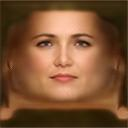
\includegraphics[width=\afifthcolumn]{img/representation/pred_tex_no_Male.jpg} &
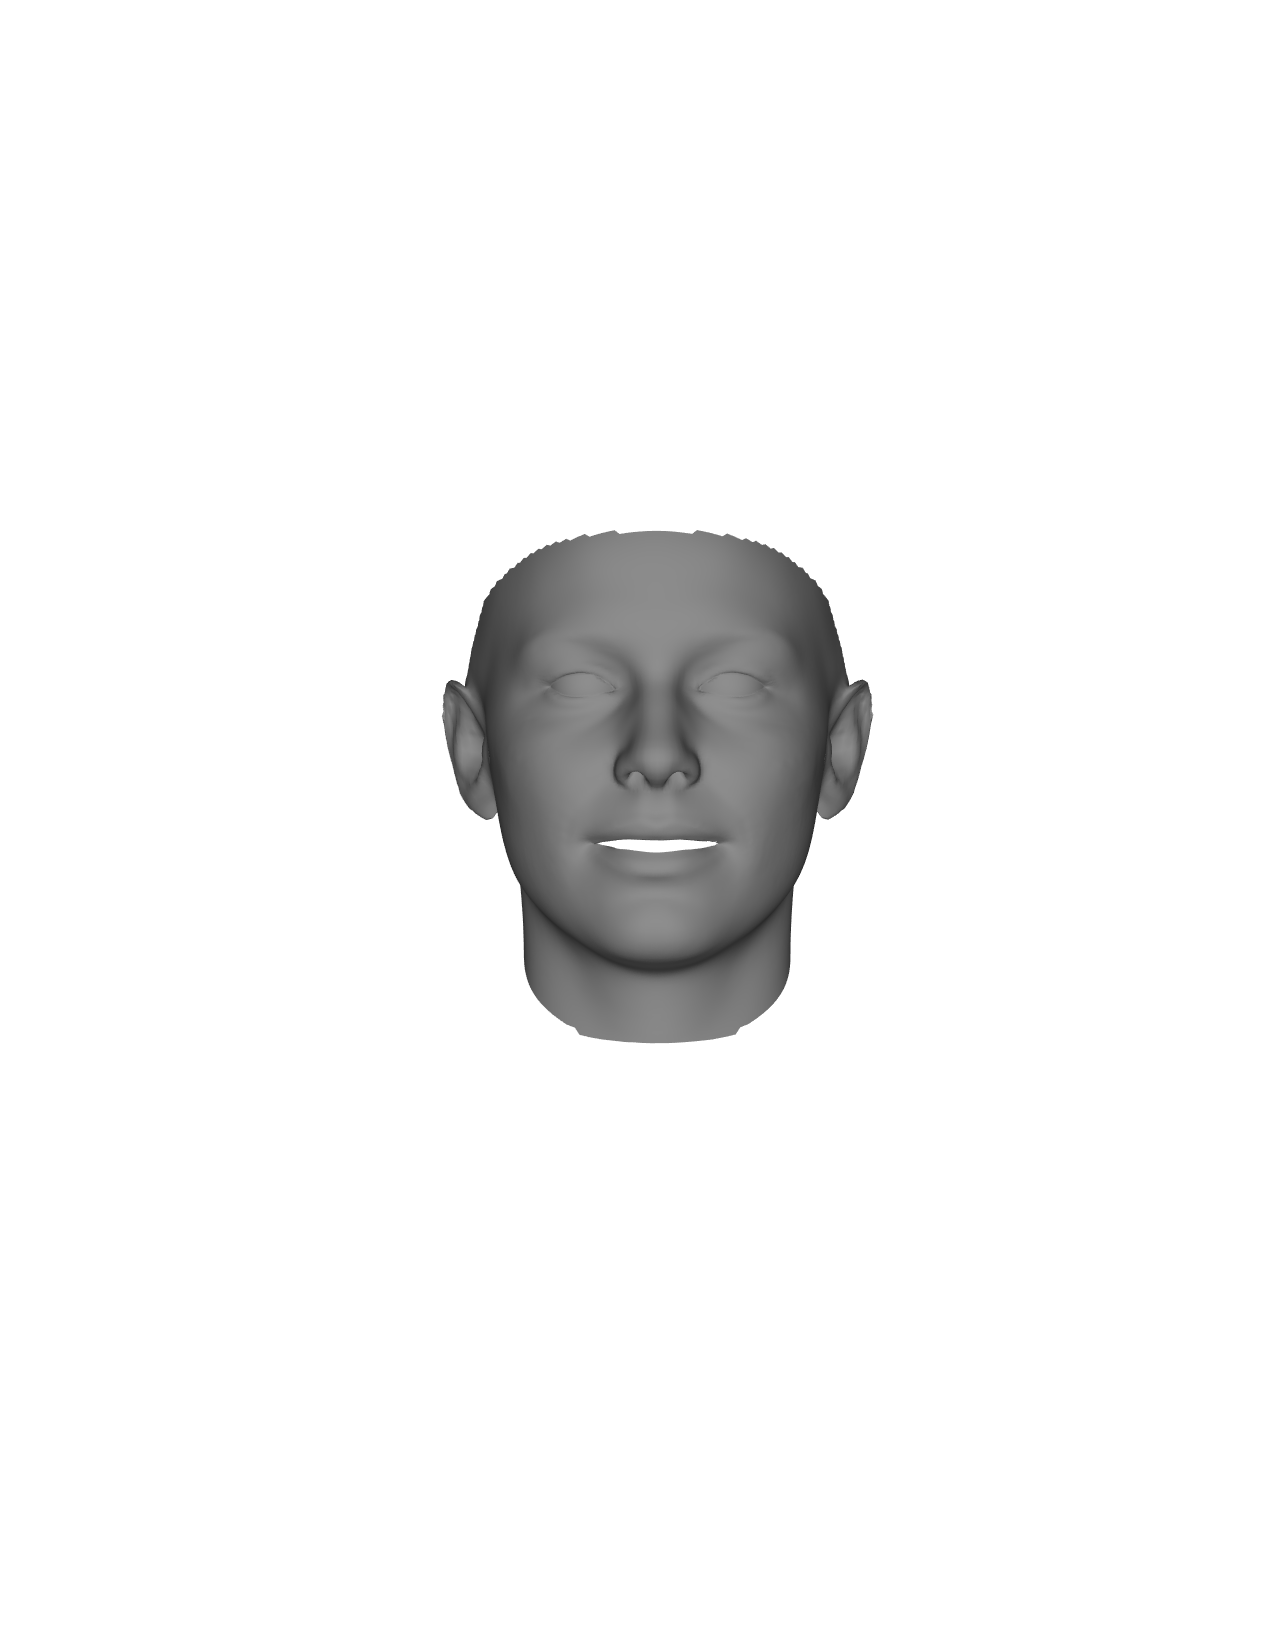
\includegraphics[trim=150 250 150 250,clip, width=\afifthcolumn]{img/representation/pred_shape_no_Male.pdf} &
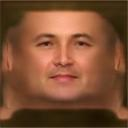
\includegraphics[width=\afifthcolumn]{img/representation/pred_tex_Chubby.jpg} &
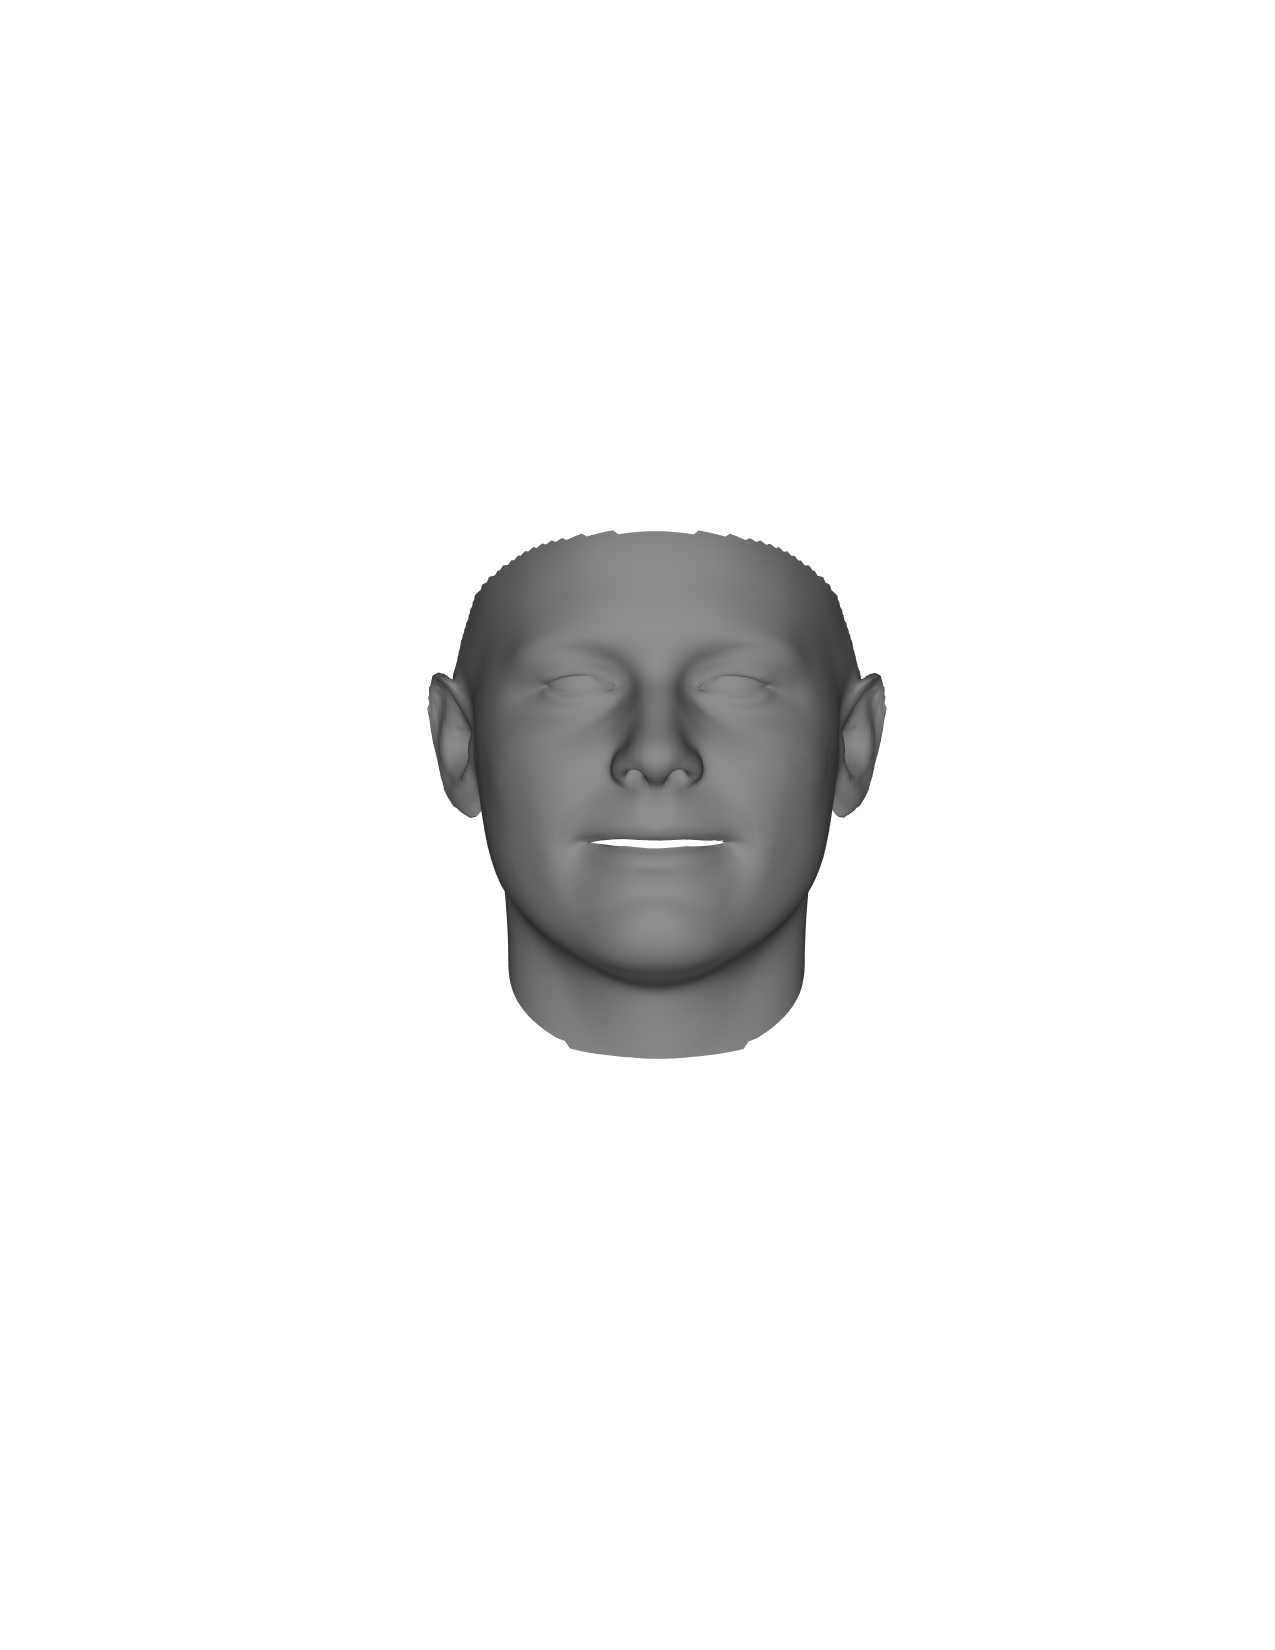
\includegraphics[trim=150 250 150 250,clip, width=\afifthcolumn]{img/representation/pred_shape_Chubby.pdf} &
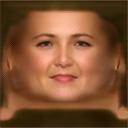
\includegraphics[width=\afifthcolumn]{img/representation/pred_tex_Smiling.jpg} &
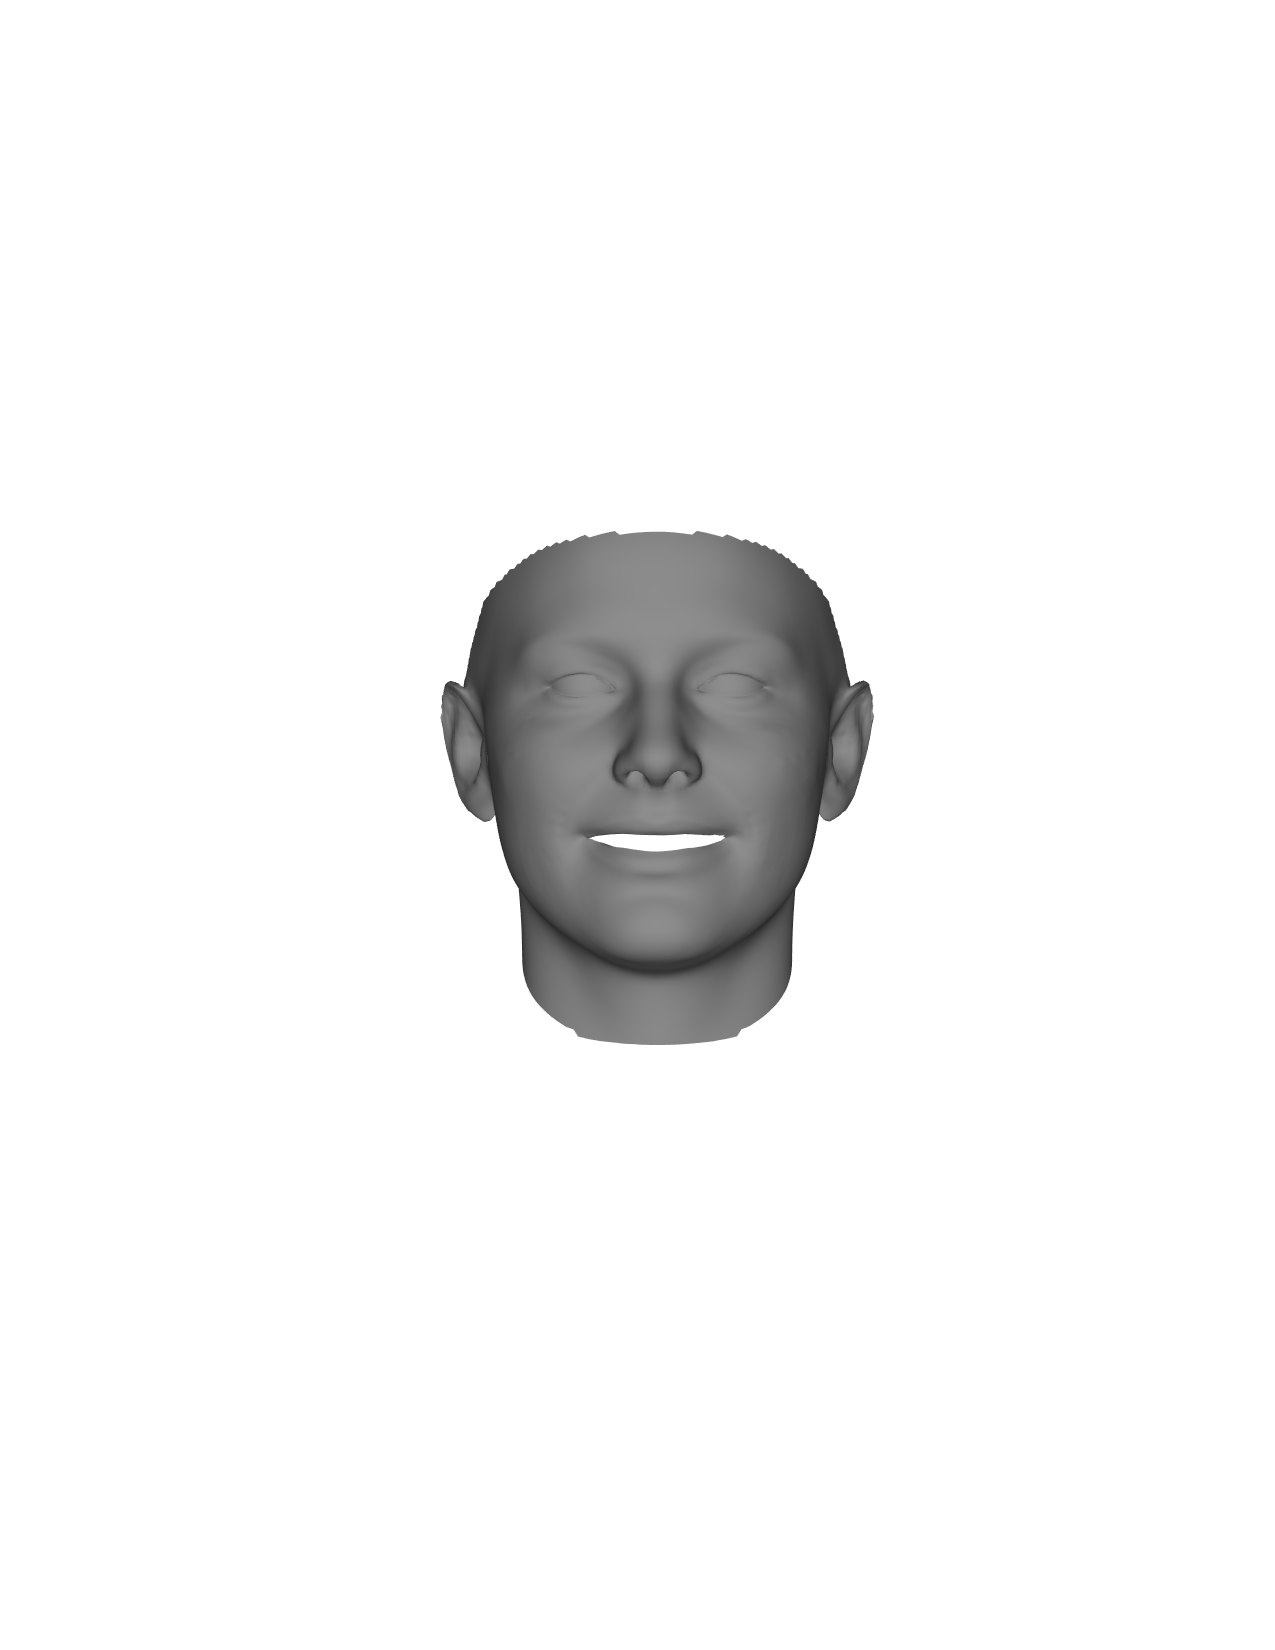
\includegraphics[trim=150 250 175 250,clip, width=\afifthcolumn]{img/representation/pred_shape_Smiling.pdf} &
\\
\multicolumn{2}{c}{Female} & \multicolumn{2}{c}{Chubby} & \multicolumn{2}{c}{Smiling} \\
%\bottomrule
\end{tabular}
\vspace{-2mm}
\caption{\small Nonlinear 3DMM generates shape and texture embedded with different attributes.}
\label{fig:meaningful_basis}\figvspace \vspace{-2mm}
\end{center}
\end{figure}






\begin{figure}[t!]
\begin{center}
\small
\setlength{\tabcolsep}{3pt}
\begin{tabular}{ @{}c@{}c@{}c@{}c@{}c@{}c@{}c@{\hskip 1.5mm}c@{}}
%\toprule
\multirow{2}{*}{Input} & \multirow{2}{*}{Linear} & \multicolumn{2}{c}{Nonlinear} \\ & & Grad desc & Network \\

\includegraphics[width=\afifthcolumn]{img/tex_grad_descent/pred_img_11_gt.jpg} &
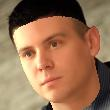
\includegraphics[trim=7 7 7 7,clip,width=\afifthcolumn]{img/tex_grad_descent/pred_img_11_linear.jpg} &

\includegraphics[width=\afifthcolumn]{img/tex_grad_descent/pred_img_11.jpg} &

\includegraphics[width=\afifthcolumn]{img/tex_grad_descent/pred_img_11_enc.jpg} &
\\

\includegraphics[width=\afifthcolumn]{img/tex_grad_descent/pred_img_30_gt.jpg} &
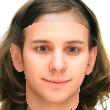
\includegraphics[trim=7 7 7 7,clip,width=\afifthcolumn]{img/tex_grad_descent/pred_img_30_linear.jpg} &
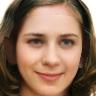
\includegraphics[width=\afifthcolumn]{img/tex_grad_descent/pred_img_30.jpg} &
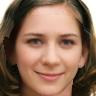
\includegraphics[width=\afifthcolumn]{img/tex_grad_descent/pred_img_30_enc.jpg} &
\\
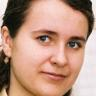
\includegraphics[width=\afifthcolumn]{img/tex_grad_descent/pred_img_45_gt.jpg} &
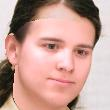
\includegraphics[trim=7 7 7 7,clip,width=\afifthcolumn]{img/tex_grad_descent/pred_img_45_linear.jpg} &
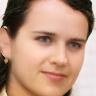
\includegraphics[width=\afifthcolumn]{img/tex_grad_descent/pred_img_45.jpg} &
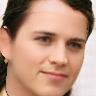
\includegraphics[width=\afifthcolumn]{img/tex_grad_descent/pred_img_45_enc.jpg} &
\\
%\bottomrule
\end{tabular}
\vspace{-2mm}
\caption{\small Texture representation power comparison. Our nonlinear model can better reconstruct the facial texture.}
\label{fig:tex_representationpower}\figvspace
\end{center}
\end{figure}

\begin{table}[t!]
\footnotesize
\caption{\small{Quantitative comparison of texture representation power.}} 
\label{tab:tex_representation_tab}
\vspace{-6mm}
\begin{center}
\begin{tabular}{ cccccccc}
\toprule 
Method & Linear & Nonlinear w.~Grad De. & Nonlinear w.~Network \\ \midrule
$L_1$    & $0.103$ & $0.066$   & $0.066$ \\ 
\bottomrule
\end{tabular}
\end{center}
\figvspace\vspace{-2mm}
\end{table}

\SubSection{Representation Power}
\Paragraph{Texture}
Given a face image, assuming we know the groundtruth shape and projection parameters, we can unwarp the texture into the UV space, as we generate ``pseudo groundtruth" texture in the weakly supervised step. 
With the groundtruth texture, by using gradient descent, we can estimate a texture parameter  $\mathbf{f}_T$ whose decoded texture matches with the groundtruth. 
Alternatively, we can minimize the reconstruction error in the image space, through the rendering layer with the groundtruth $\mathbf{S}$ and $\mathbf{m}$. 
Empirically, the two methods give similar performances but we choose the first option as it involves only one warping step, instead of rendering in every optimization iteration.
For the linear model, we use the fitting results of Basel texture and Phong illumination model~\cite{phong1975illumination} given by~\cite{zhu2016face}. 
As in Fig.~\ref{fig:tex_representationpower}, our nonlinear texture is closer to the groundtruth than the linear model, especially for in-the-wild images (the first two rows).
This is expected since the linear model is trained with controlled images. 
Quantitatively, our nonlinear model has significantly lower $L_1$ reconstruction error than the linear model ($0.066$ vs.~$0.103$, as in Tab.~\ref{tab:tex_representation_tab}).


\begin{figure}[t!]
\begin{center}
\small
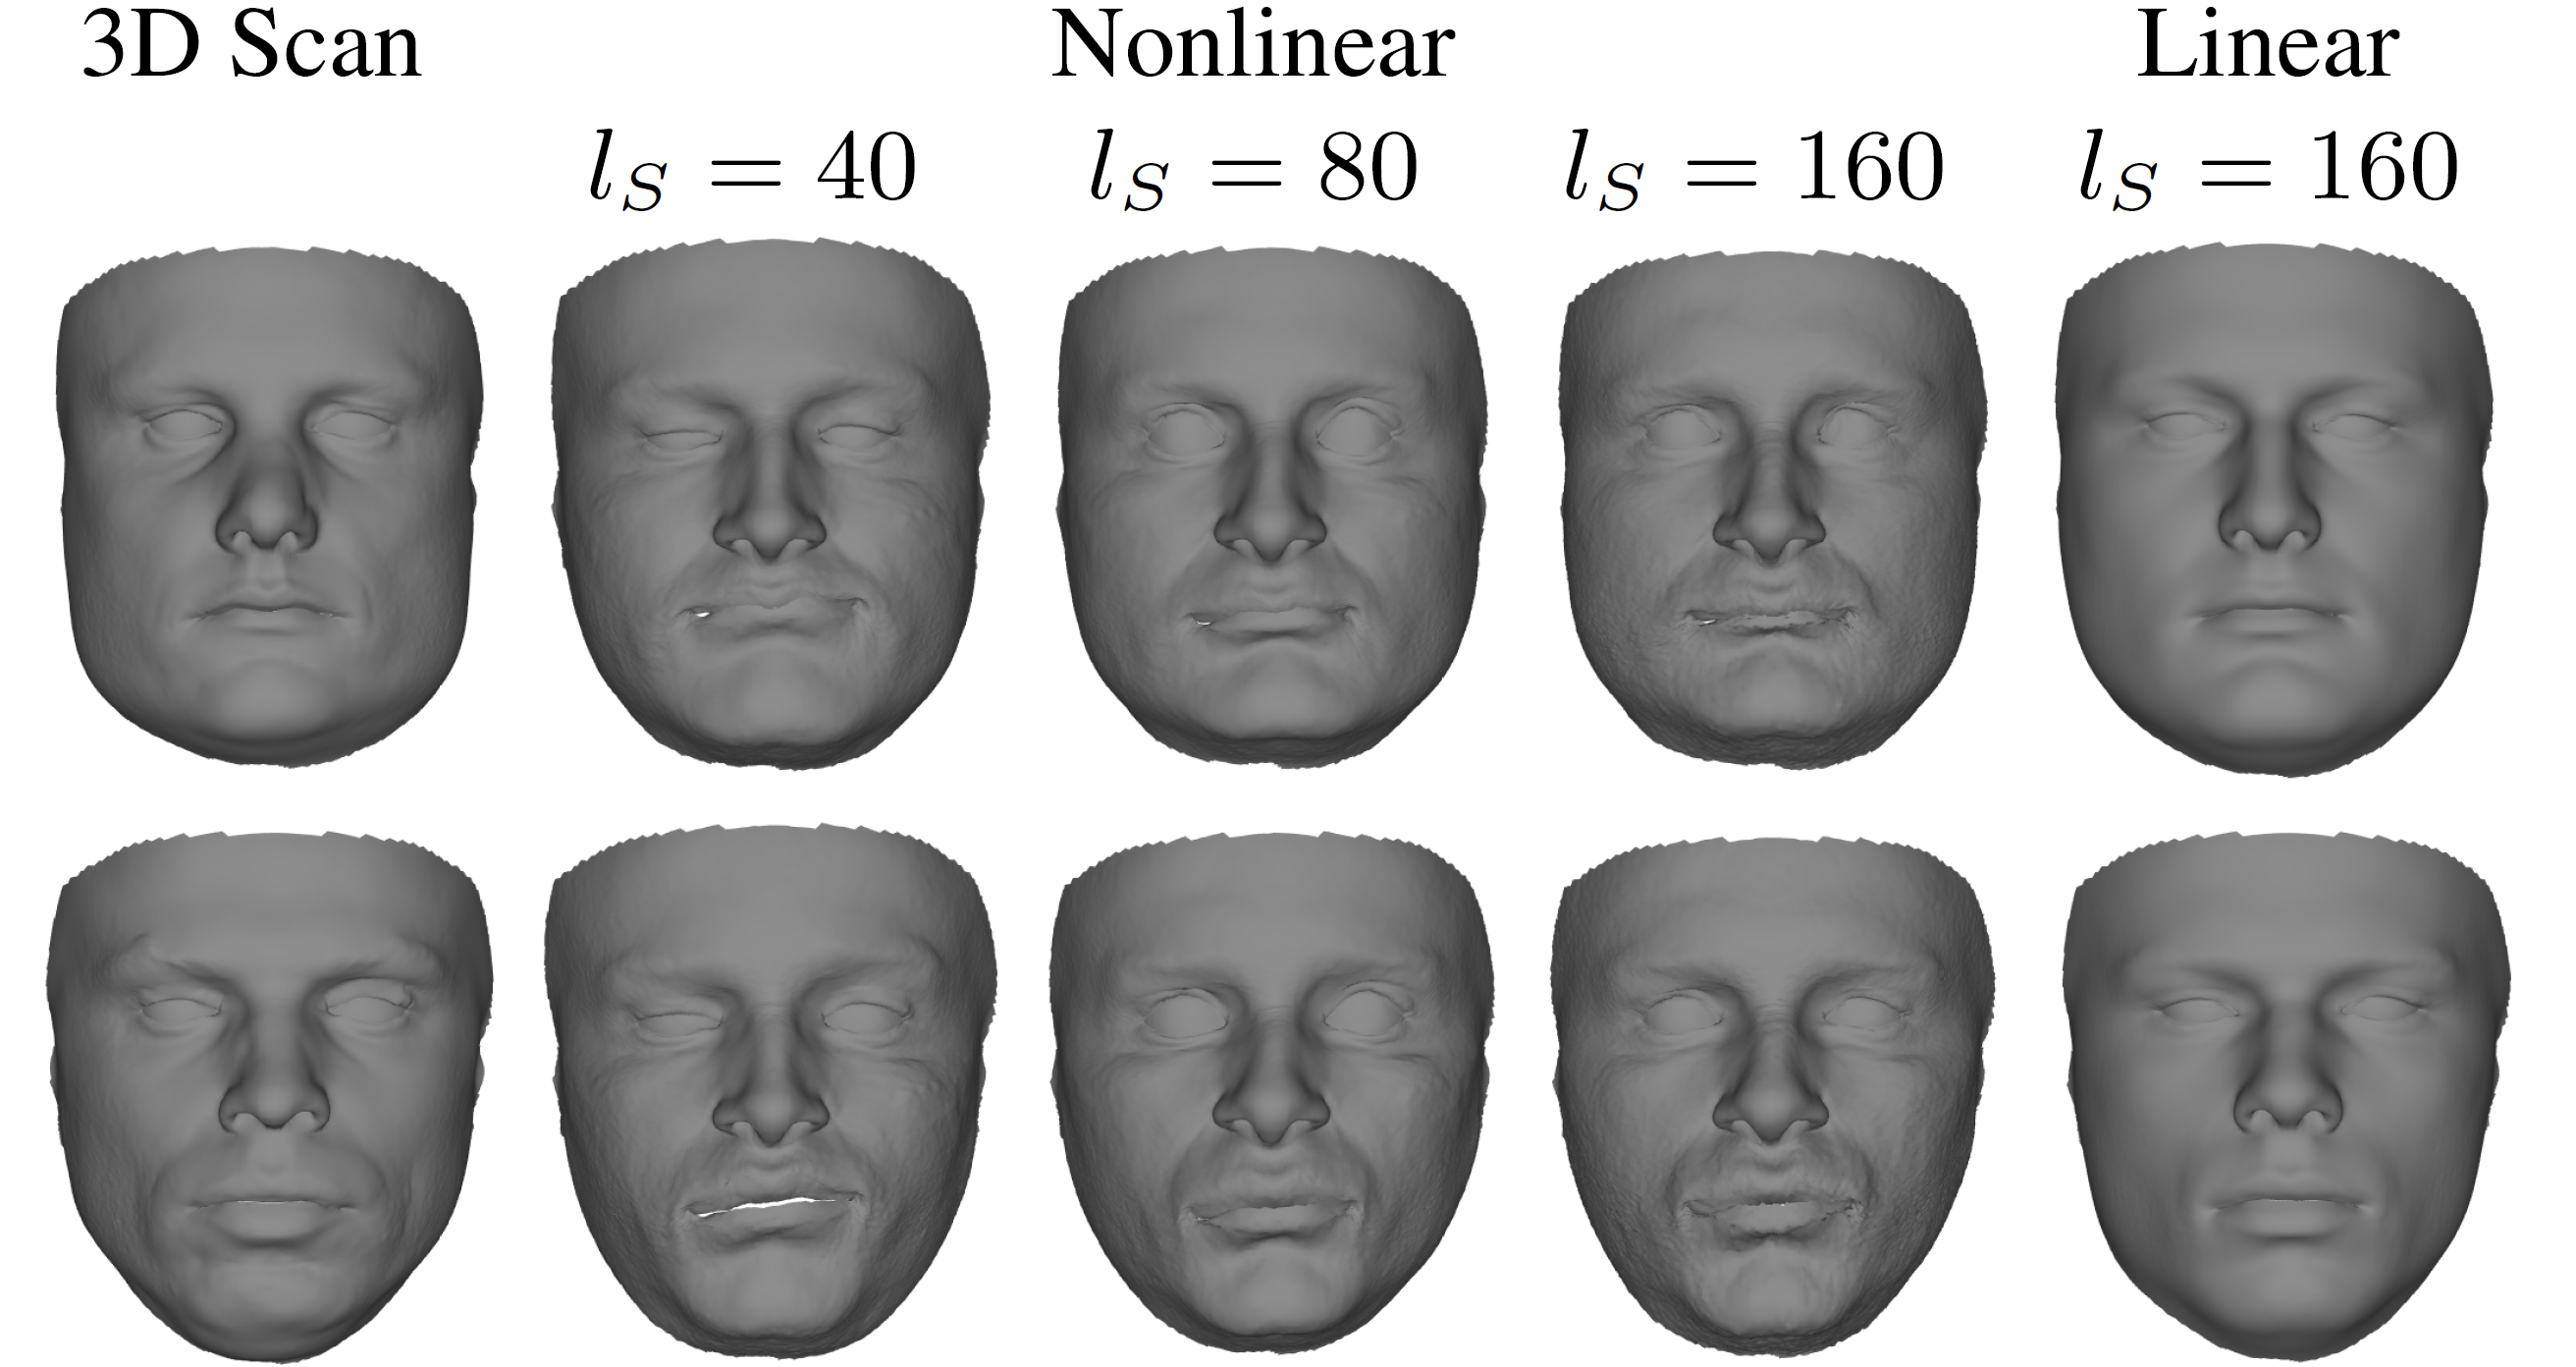
\includegraphics[trim = 0 0 0 0, clip, width=0.95\linewidth]{./img/results/BU-4DFE/Linear_vs_Nonlinear.png}
\figvspace\vspace{1mm}
\caption{\small Shape representation power comparison.}
\label{fig:shape_representation}\figvspace
\end{center}
\end{figure}



\Paragraph{3D Shape}
We also compare the power of nonlinear and linear 3DMM in representing real-world 3D scans. 
We compare with BFM~\cite{paysan20093d}, the most commonly used 3DMM at present. 
We use ten 3D face scans provided by~\cite{paysan20093d}, which are not included in the training set of BFM.
As these face meshes are already registered using the same triangle definition with BFM,  no registration is necessary.
%
Given the groundtruth shape, by using gradient descent, we can estimate a shape parameter whose decoded shape matches the groundtruth. 
We define matching criteria on both vertex distances and surface normal direction. 
This empirically improves fidelity of final results compared to only optimizing vertex distances.
Also, to emphasize the compactness of nonlinear models, we train different models with different latent space sizes.
%
Fig.~\ref{fig:shape_representation} shows the visual quality of two models' reconstructions.
As we can see, our reconstructions closely match the face shapes. 
Meanwhile the linear model struggles with face shapes outside its PCA span.

To quantify the difference, we use NME, averaged per-vertex errors between the recovered and groundtruth shapes, normalized by inter-ocular distances. 
Our nonlinear model has a significantly smaller reconstruction error than the linear model, $0.0196$ vs.~$0.0241$ (Tab.~\ref{tab:shape_representation_number}). 
Also, the non-linear models are more compact. 
They can achieve similar performances as linear models whose latent space’s sizes doubled.

\begin{table}[t!]
\footnotesize
\caption{\small{3D scan reconstruction comparison (NME).}} 
\label{tab:shape_representation_number}
\vspace{-6mm}
\begin{center}
\begin{tabular}{ cccccccc}
\toprule 
$l_S$     & $40$ & $80$ & $160$ \\ \midrule
Linear    & $0.0321$ & $0.0279$ & $0.0241$ \\
Nonlinear & $0.0277$ & $0.0236$ & $\mathbf{0.0196}$ \\
\bottomrule
\end{tabular}
\end{center}
\figvspace
\end{table}



\begin{figure}[t!]
\begin{center}
\small
\setlength{\tabcolsep}{3pt}
\begin{tabular}{ @{\hskip 1.5mm}c@{\hskip 1.5mm}c@{\hskip 1.5mm}c@{\hskip 1.5mm}c@{}c@{}c@{}c@{\hskip 1.5mm}c@{}}
%\toprule
Input & Shape & Texture & Reconstruction \\
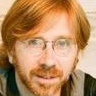
\includegraphics[width=\FittingFigWid]{img/results/CelebA/pred_CelebA_tex_118_in.png} &
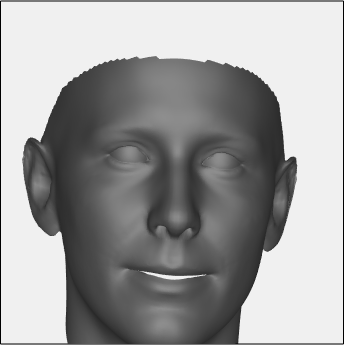
\includegraphics[trim=3 3 3 3,clip,width=\FittingFigShapeWid]{img/results/CelebA/pred_CelebA_shape_118.png} &
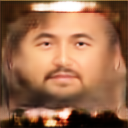
\includegraphics[width=\FittingFigWid]{img/results/CelebA/pred_CelebA_tex_118.png} &
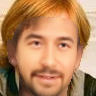
\includegraphics[width=\FittingFigWid]{img/results/CelebA/pred_CelebA_tex_118_img.png} &
\\
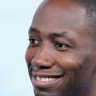
\includegraphics[width=\FittingFigWid]{img/results/CelebA/pred_CelebA_tex_133_in.png} &
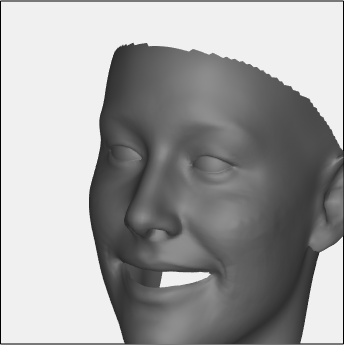
\includegraphics[trim=3 3 3 3,clip,width=\FittingFigShapeWid]{img/results/CelebA/pred_CelebA_shape_133.png} &
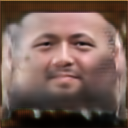
\includegraphics[width=\FittingFigWid]{img/results/CelebA/pred_CelebA_tex_133.png} &
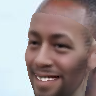
\includegraphics[width=\FittingFigWid]{img/results/CelebA/pred_CelebA_tex_133_img.png} &
\\
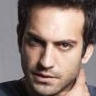
\includegraphics[width=\FittingFigWid]{img/results/CelebA/pred_CelebA_tex_159_in.png} &
\includegraphics[trim=3 3 3 3,clip,width=\FittingFigShapeWid]{img/results/CelebA/pred_CelebA_shape_159.png} &
\includegraphics[width=\FittingFigWid]{img/results/CelebA/pred_CelebA_tex_159.png} &
\includegraphics[width=\FittingFigWid]{img/results/CelebA/pred_CelebA_tex_159_img.png} &
\\
\includegraphics[width=\FittingFigWid]{img/results/CelebA/pred_CelebA_tex_245_in.png} &
\includegraphics[trim=3 3 3 3,clip,width=\FittingFigShapeWid]{img/results/CelebA/pred_CelebA_shape_245.png} &
\includegraphics[width=\FittingFigWid]{img/results/CelebA/pred_CelebA_tex_245.png} &
\includegraphics[width=\FittingFigWid]{img/results/CelebA/pred_CelebA_tex_245_img.png} &
\\
%\bottomrule
\end{tabular}
\vspace{-2mm}
\caption{\small 3DMM fits to faces with diverse skin color, pose, expression, lighting, facial hair, and faithfully recovers these cues.}
\label{fig:3dmm_fitting}\figvspace
\end{center}
\end{figure}



\begin{figure}[t!]
\begin{center}
\small
\setlength{\tabcolsep}{3pt}
\begin{tabular}{ @{\hskip 1.5mm}c@{\hskip 1.5mm}c@{\hskip 1.5mm}c@{\hskip 1.5mm}c@{}c@{}c@{}c@{\hskip 1.5mm}c@{}}
%\toprule 1086 452 1159 450
\includegraphics[width=\AlignFigWid]{img/results/AFLW2000/_pred_AFLW2000_landmarkoverlay_1086.png} &
\includegraphics[width=\AlignFigWid]{img/results/AFLW2000/_pred_AFLW2000_landmarkoverlay_452.png} &
\includegraphics[width=\AlignFigWid]{img/results/AFLW2000/_pred_AFLW2000_landmarkoverlay_1159.png} &
\includegraphics[width=\AlignFigWid]{img/results/AFLW2000/_pred_AFLW2000_landmarkoverlay_450.png} &
\\
\includegraphics[width=\AlignFigWid]{img/results/AFLW2000/_pred_AFLW2000_overlay_1086.jpg} &
\includegraphics[width=\AlignFigWid]{img/results/AFLW2000/_pred_AFLW2000_overlay_452.jpg} &
\includegraphics[width=\AlignFigWid]{img/results/AFLW2000/_pred_AFLW2000_overlay_1159.jpg} &
\includegraphics[width=\AlignFigWid]{img/results/AFLW2000/_pred_AFLW2000_overlay_450.jpg} &
\\
%\bottomrule
\end{tabular}
\vspace{-2mm}
\caption{\small Our 2D face alignment results. Invisible landmarks are marked as red. We can handle extreme pose and/or expression. }
\label{fig:2d_align}\figvspace \vspace{-2mm}
\end{center}
\end{figure}




\begin{table}[t!]
\footnotesize
\caption{\small{Face alignment performance on ALFW2000}} 
\label{tab:2d_face_align}
\vspace{-6mm}
\begin{center}
\begin{tabular}{ cccccccc}
\toprule 
Method & Linear & SDM~\cite{yan2013learn} & 3DDFA~\cite{zhu2016face} & Ours \\ \midrule
NME    & $5.61$ & $6.12$                  & $5.42$                   & $\mathbf{4.70}$ \\ 
\bottomrule
\end{tabular}
\end{center}
\figvspace\vspace{-2mm}
\end{table}



\begin{figure*}[t!]
\begin{center}
\small
\setlength{\tabcolsep}{3pt}
\begin{tabular}{c@{\hskip 1.5mm}c@{\hskip 1mm}c@{\hskip 1.5mm}c@{\hskip 1mm}c@{\hskip 1.5mm}c@{\hskip 1mm}c@{\hskip 1mm}c@{}}
%\toprule
Input & \multicolumn{2}{c}{Our}  & \multicolumn{2}{c}{Richardson16} & \multicolumn{2}{c}{Tewari17} \\
\includegraphics[width=\FittingFigWid]{img/Random/300VW_1_in.png} &
\includegraphics[width=\FittingFigWid]{img/Random/300VW_1_rescon.png} &
\includegraphics[width=\FittingFigWid]{img/Random/300VW_1_shape.png} &
\includegraphics[width=\FittingFigWid]{img/Random/300VW_1_Richardson_rescon.png} &
\includegraphics[width=\FittingFigWid]{img/Random/300VW_1_Richardson_shape.png} &
\includegraphics[width=\FittingFigWid]{img/Random/300VW_1_Tewari_rescon.png} &
\includegraphics[width=\FittingFigWid]{img/Random/300VW_1_Tewari_shape.png} &
\\
\includegraphics[width=\FittingFigWid]{img/Random/300VW_7_in.png} &
\includegraphics[width=\FittingFigWid]{img/Random/300VW_7_rescon.png} &
\includegraphics[width=\FittingFigWid]{img/Random/300VW_7_shape.png} &
\includegraphics[width=\FittingFigWid]{img/Random/300VW_7_Richardson_rescon.png} &
\includegraphics[width=\FittingFigWid]{img/Random/300VW_7_Richardson_shape.png} &
\includegraphics[width=\FittingFigWid]{img/Random/300VW_7_Tewari_rescon.png} &
\includegraphics[width=\FittingFigWid]{img/Random/300VW_7_Tewari_shape.png} &
\\
%\bottomrule
\end{tabular}
\vspace{-2mm}
\caption{\small 3D reconstruction results comparison. We achieve comparable visual quality in 3D reconstruction.}
\label{fig:3drecon_exp}\figvspace \vspace{-2mm}
\end{center}
\end{figure*}

\begin{figure}[t!]
\centering
\includegraphics[trim=10 22 25 12,clip,width=\linewidth]{img/3D_rescon_quan.png}
\vspace{-4mm}
\caption{\small Quantitative evaluation of 3D reconstruction. We obtain a low error that is comparable to optimization-based methods.}
\label{fig:3d_rescon_quan}
\figvspace 
\end{figure}



\SubSection{Applications}
Having shown the capability of our nonlinear 3DMM (i.e., two decoders), now we demonstrate the applications of our entire network, which has the additional encoder.
Many applications of 3DMM are centered on its ability to fit to 2D face images.
%
Fig.~\ref{fig:3dmm_fitting} visualizes our 3DMM fitting results on CelebA dataset. 
Our encoder estimates the shape $\mathbf{S}$, texture $\mathbf{T}$ as well as projection parameter $\mathbf{m}$. 
We can recover personal facial characteristic in both shape and texture. 
Our texture can have variety skin color or facial hair, which is normally hard to be recovered by linear 3DMM.

\Paragraph{2D Face Alignment}
Face alignment is a critical step for any facial analysis task such as face recognition. 
With enhancement in the modeling, we hope to improve this task (Fig.~\ref{fig:2d_align}). 
We compare face alignment performance with state-of-the-art methods, SDM~\cite{yan2013learn} and 3DDFA~\cite{zhu2016face}, on the AFLW2000 dataset. 
The alignment accuracy is evaluated by the Normalized Mean Error (NME), the average of visible landmark error normalized by the bounding box size.
Here, current state-of-the-art 3DDFA~\cite{zhu2016face} is a cascade of CNNs that iteratively refines its estimation in multiple steps, meanwhile ours is a single-pass of $E$ and $D_S$. 
However, by jointly learning model fitting with 3DMM, our network can surpass ~\cite{zhu2016face}'s performance, as in Tab.~\ref{tab:2d_face_align}.
Another perspective is that in conventional 3DMM fitting~\cite{zhu2016face}, the texture is used as the input to regress the shape parameter, while ours adopts an analysis-by-synthesis scheme and texture is the output of the synthesis.
Further, for a more fair comparison of nonlinear vs.~linear models, we train an encoder with the same architecture as our $E$, whose output parameter will multiple with the linear shape bases $\mathbf{A}$, and train with the landmark loss function (Eqn.~\ref{eq:landmarkloss}). 
Again we observe the higher error from the linear model-based fitting.

\Paragraph{3D Face Reconstruction}
We compare our approach to recent works: the CNN-based iterative supervised regressor of Richardson et al.~\cite{richardson20163d, richardson2017learning} and unsupervised regressor method of Tewari et al.~\cite{tewari2017mofa}.
The work by Tewari et al.~\cite{tewari2017mofa} is relevant to us as they also learn to fit 3DMM in an unsupervised fashion. 
However, they are limited to linear 3DMM bases, which of course are not jointly trained with the model. 
Also, we only compare with the coarse network in~\cite{richardson2017learning} as their refinement network use SfS, which leads to a 2.5D representation and loses correspondence between different 3D shapes. 
This is orthogonal to our approach.
Fig.~\ref{fig:3drecon_exp} shows visual comparison. 
Following the same setting in~\cite{tewari2017mofa}, we also quantitatively compare our method with prior works on $9$ subjects of FaceWarehouse database~(Fig.~\ref{fig:3d_rescon_quan}). 
We achieve on-par results with Garrido et al.~\cite{garrido2016reconstruction}, an offline optimization method, while surpassing all other regression methods~\cite{tran2017regressing, richardson2017learning, tewari2017mofa}.


\begin{figure}[t!]
\begin{center}
\small
\setlength{\tabcolsep}{3pt}
\begin{tabular}{c@{\hskip 1.5mm}c@{\hskip 1mm}c@{\hskip 1.5mm}c@{\hskip 1mm}c@{\hskip 1.5mm}c@{\hskip 1mm}c@{\hskip 1mm}c@{}}
%\toprule
Input & No GAN & ImgGAN& PatchGAN \\
\includegraphics[width=\AblTexFigWid]{img/Ablation/Input1.png} &
\includegraphics[width=\AblTexFigWid]{img/Ablation/ImgNoGAN1.png} &
\includegraphics[width=\AblTexFigWid]{img/Ablation/ImgGAN1.png} &
\includegraphics[width=\AblTexFigWid]{img/Ablation/PatchGAN1.png} &
\\
\includegraphics[width=\AblTexFigWid]{img/Ablation/Input2.png} &
\includegraphics[width=\AblTexFigWid]{img/Ablation/ImgNoGAN2.png} &
\includegraphics[width=\AblTexFigWid]{img/Ablation/ImgGAN2.png} &
\includegraphics[width=\AblTexFigWid]{img/Ablation/PatchGAN2.png} &
%\bottomrule
\end{tabular}
\vspace{-2mm}
\caption{\small Effects of adversarial losses for texture learning.}
\label{fig:abl_tex}
\figvspace \vspace{-2mm}
\end{center}
\end{figure}

\SubSection{Ablation on Texture Learning}
With great representation power, we would like to learn a realistic texture model from in-the-wild images. 
The rendering layer opens a possibility to apply adversarial loss in addition to global $L_1$ loss. 
%
Using a global image-based discriminator is redundant as the global structure is guaranteed by the rendering layer. 
Also, we empirically find that using global image-based discriminator can cause severe artifacts in the resultant texture. 
Fig.~\ref{fig:abl_tex} visualizes outputs of our network with different options of adversarial loss. 
Clearly, patchGAN offers higher realism and fewer artifacts.
